\documentclass{beamer}
\usepackage[utf8]{inputenc}
\usepackage{graphicx}
\author[Sowmya Vajjala]{Instructor: Sowmya Vajjala}

\title[LING 410X]{LING 410X: Language as Data}
\subtitle{Semester: Spring '18}

\date{10 Apr 2018}

\institute{Iowa State University, USA}
%%%%%%%%%%%%%%%%%%%%%%%%%%%

\begin{document}

\begin{frame}\titlepage
\end{frame}

\begin{frame}
\frametitle{Class Outline}
\begin{itemize}
\item Assignment 5 and project initial submission - comments
\item Discussion on Stylo
\item Clustering - overview
%\item Rolling Delta - how does it work?
\item One example application of stylo for non-literature analysis
\end{itemize}
\end{frame}


\begin{frame}
\frametitle{Assignment 5 - some comments}
\begin{itemize}
\item How long did it take for you to run the program as is?
$\Rightarrow$ 15 min to 1 hour \pause
\item With some customized pre-processing, you may see more meaningful topic clusters than default.
\begin{itemize}
\item adding custom stopwords, increasing to 8-10 topics seem to make more sense.
\item note: stemming is less interpretable for humans.
\end{itemize} \pause 
\item There were some strange characters in the topics, most frequent words. One possible solution: reading the text as utf8?
\end{itemize}
\end{frame}

\begin{frame}
\frametitle{Some other observations}
\begin{itemize}
\item ngram models: May result in better modeling, but will increase vocabulary size and training time. \pause
\item topic models vs word clouds: topic models give more information than word clouds \pause
\end{itemize}
\end{frame}

\begin{frame}
\frametitle{Where are topic models useful?}
\begin{itemize}
\item Creating topic distribution for research articles, political speeches, tweets etc
\item Comparing topics covered in different newspapers from different regions of US. 
\item To detect “hottest” topics in a certain time frame
\item Understanding system logs to know about bug patterns
\item Knowing customer reactions to a product, Market demands over time etc.
\item Find themes inside large collections of texts
\item Using with non-text data (music recommendation, image classification etc)
\end{itemize}
\end{frame}

\begin{frame}
\frametitle{Your project ideas}
\begin{itemize}
\item In general, ideas are good, and come from your own discplines.
\item Some people wrote in detail (with alternative plans) and some wrote like 1 paragraph.
\item More details is good for you
\end{itemize}
\end{frame}


\begin{frame}
\frametitle{Clarification regarding dead-week}
Final exam for this course = Your submission of final project reports. Project presentations do not count as final exam. \\
\footnotesize \medskip
"Final exams may not be given at a time other than that for which the exam is scheduled by the registrar. An instructor may not give a final exam prior to final exam week nor change the time of offering of the final examination as it appears in the final exam schedule. Permission to change the time for which an exam is scheduled may be given only by the dean of the college. If the instructor elects not to give a final exam in a course of two or more credits, the class is required to meet at the scheduled final exam period for other educational activity such as a review of the course or feedback on previous exams."  Note that additional policies and scheduling processes apply to final exams that are given in the online testing center."
\end{frame}


\begin{frame}
\frametitle{}
\Large Working with stylo - some observations 
\end{frame}


\begin{frame}
\frametitle{Using stylo for comparing writing style - 1}
\begin{itemize}
\item Using bigrams showed based results - Dickens and Strindberg had one cluster each. Chekhov 2--4 was one cluster and Ibsen1 and Chekhov1 came as another cluster.
\item Setting ngram as 2 or changing MFW setting did not show any change. 
\item Classic delta distance perform better than Euclidean distance and cosine distance for this text data.
\end{itemize}
\end{frame}

\begin{frame}
\frametitle{Using stylo for comparing writing style - 2}
ngrams 1 vs ngrams 5 - very different clusters. 
\begin{tabular}{cc}
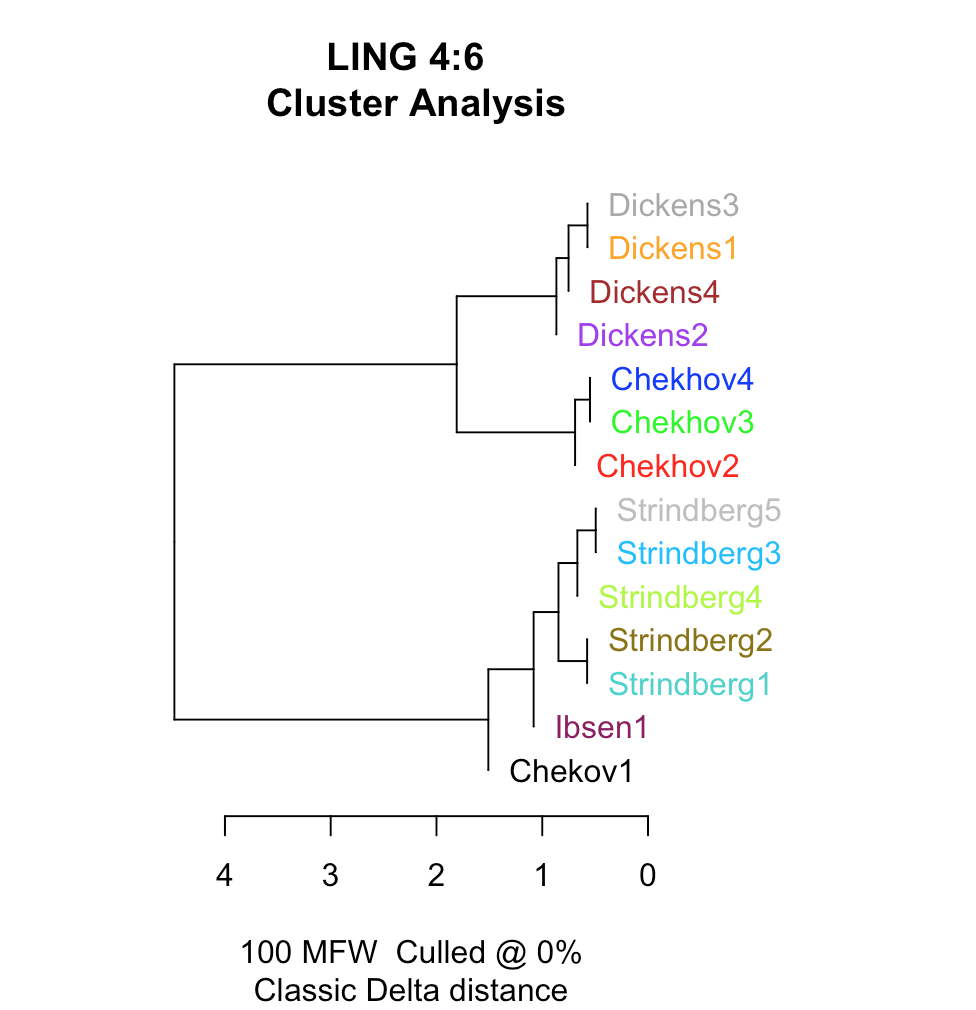
\includegraphics[width=0.4\textwidth]{spoth-100mfw.jpg} & 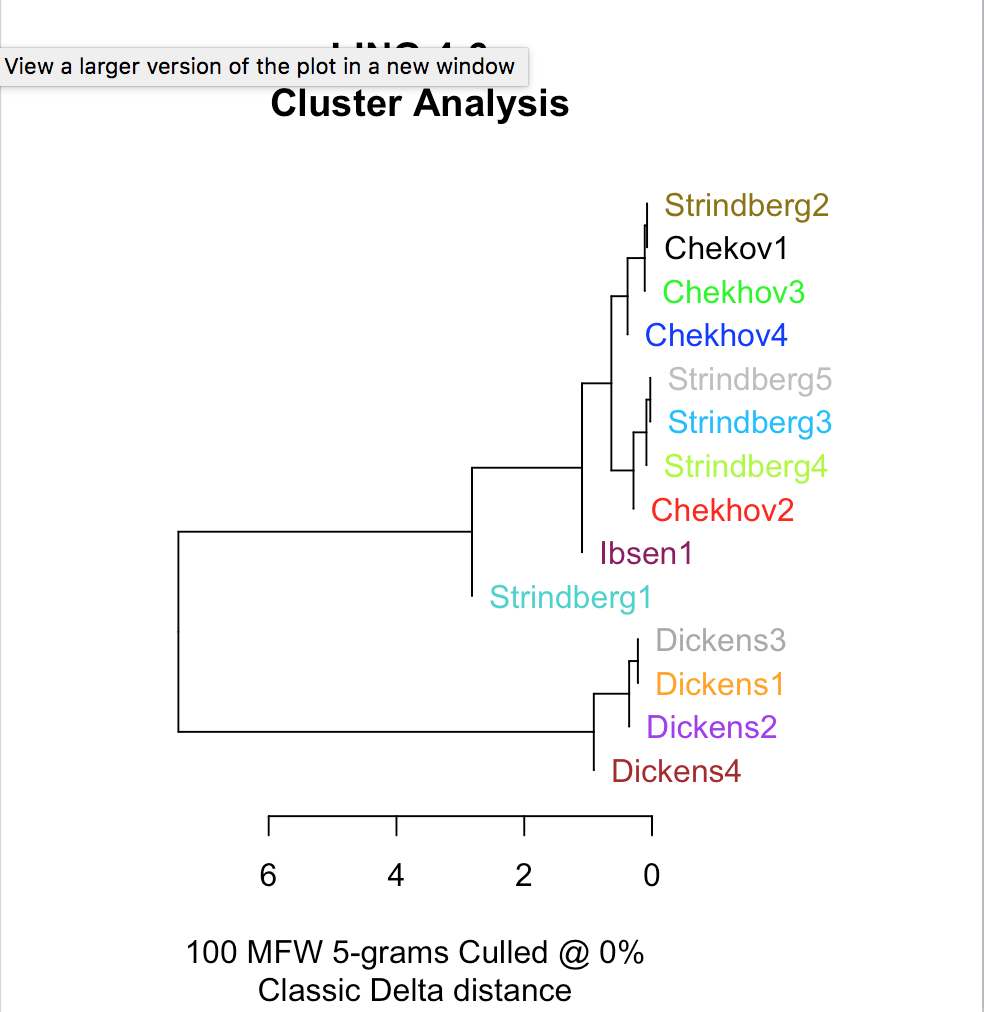
\includegraphics[width=0.4\textwidth]{spoth-100mfw-5grams.jpg}\\
\end{tabular}
\end{frame}

\begin{frame}
\frametitle{Using stylo for comparing writing style - 3}
ngrams 1 vs ngrams 3. 
\begin{tabular}{cc}
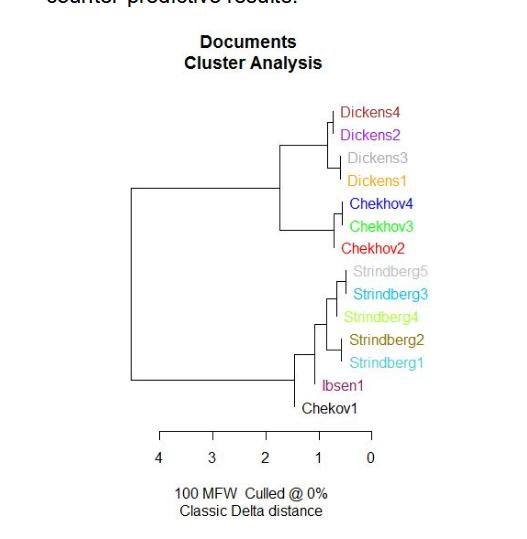
\includegraphics[width=0.4\textwidth]{cockrill-1.png} & 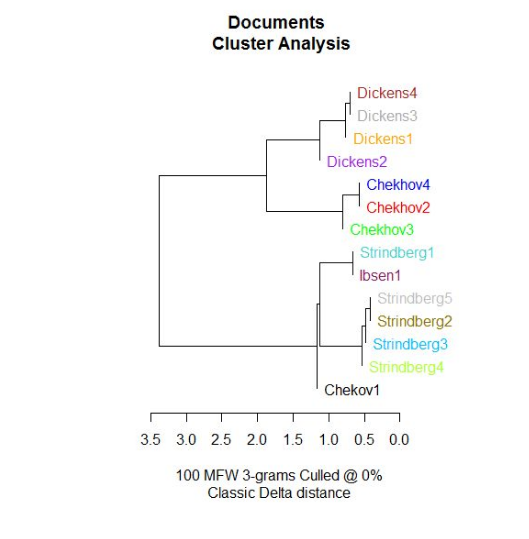
\includegraphics[width=0.4\textwidth]{cockrill-2.png}\\
\end{tabular}
\\ choosing 1000 MFW showed best cluster.
\end{frame}

\begin{frame}
\frametitle{Using Stylo for comparing writing style - 4}
\begin{itemize}
\item Cluster analysis changes with different settings (MFW, ngrams etc)
\item Bootstrap consensus trees, another cluster visualization method, is perhaps a better way. 
\end{itemize}
\end{frame}

\begin{frame}
\frametitle{}
\Large Clustering - overview
\end{frame}

\begin{frame}
\frametitle{Process}
\begin{itemize}
\item Let us say I have a collection of texts.
\item I choose to represent the collection of texts as a feature vector (say, taking 500 most frequent words in the corpus as my features).
\item Now, if i can represent each document like this, I should be able to compare two documents based on how far away their feature vectors are from each other.
\item If I start with considering each document as its own cluster, and step by step, group documents that are "close" to each other, you end up with one large cluster for entire data 
\end{itemize}
(Consider a space of only two words as features - to visualize the notion of document similarity)
\end{frame}

\begin{frame}
\frametitle{The Measure of Closeness}
%Mention Delta and give an overview
\begin{itemize}
\item We need some way of measuring the closeness or similarity, if we want to group texts together. One such measure Burrows' Delta (Burrows, 2002). 
\item What is that?
\begin{itemize}
\item Let us assume a collection of texts, and we want to study their stylistic differences, using $n$ most frequent words in the collection.
\item Now, each Document \textit{D} can be represented by a vector: ($f_1$(D), $f_2$(D) ... $f_n$(D)) of the frequency of occurrence of all frequent words.
\item If we scale the feature vector, to normalize the values, each $f_i$(D) for a document D becomes equal to a new value $z_i$(D)  which is defined as: ($f_i$(D) - $\mu$)/$\sigma$
\\ (where $\mu$ is the mean of the distribution of $f_i$ across all documents in the corpus)
\item So, the new representation for a document is: D = ($z_1$(D), $z_2$(D) ... $z_n$(D))
%\item Now, burrows Delta between two documents D1 and D2 is defined as the distance between these 
\end{itemize}
\end{itemize}
\end{frame}

\begin{frame}
\frametitle{Burrows Delta}
If we have two documents D1 and D2, represented as ($z_1$(D1), $z_2$(D1) ... $z_n$(D1)) and ($z_1$(D2), $z_2$(D2) ... $z_n$(D2)) respectively, Burrows Delta is given by:
$\Delta_B$ = $|z(D1) -z(D2)|$ (i.e., this is the "Manhattan Distance" between these two normalized feature vectors).
\end{frame}

\begin{frame}
\frametitle{Different formulae}
\begin{itemize}
\item Different variations of Delta exist, based on how the normalized representations for documents are formed, and what measure of distance is used on the normalized representations. 
\item Examples: Argamon's Delta (square of the $\Delta_B$ value in the previous slide), Eder's Delta etc.
\item Calculating distances without the normalization step using Manhattan distance, Euclidean distance, Canberra distance etc.
\end{itemize}
\end{frame}

\begin{frame}
\frametitle{Problem with clusters}
\begin{itemize}
\item sensitive to the initial choices (e.g., distance measure, number of features)
\item any change for those settings may result in drastically different clusters.
\item ... so, inconsistent.
\end{itemize}
\end{frame}

\begin{frame}
\frametitle{Overcoming this problem with clusters}
Build multiple clusters and compare. 
\\ 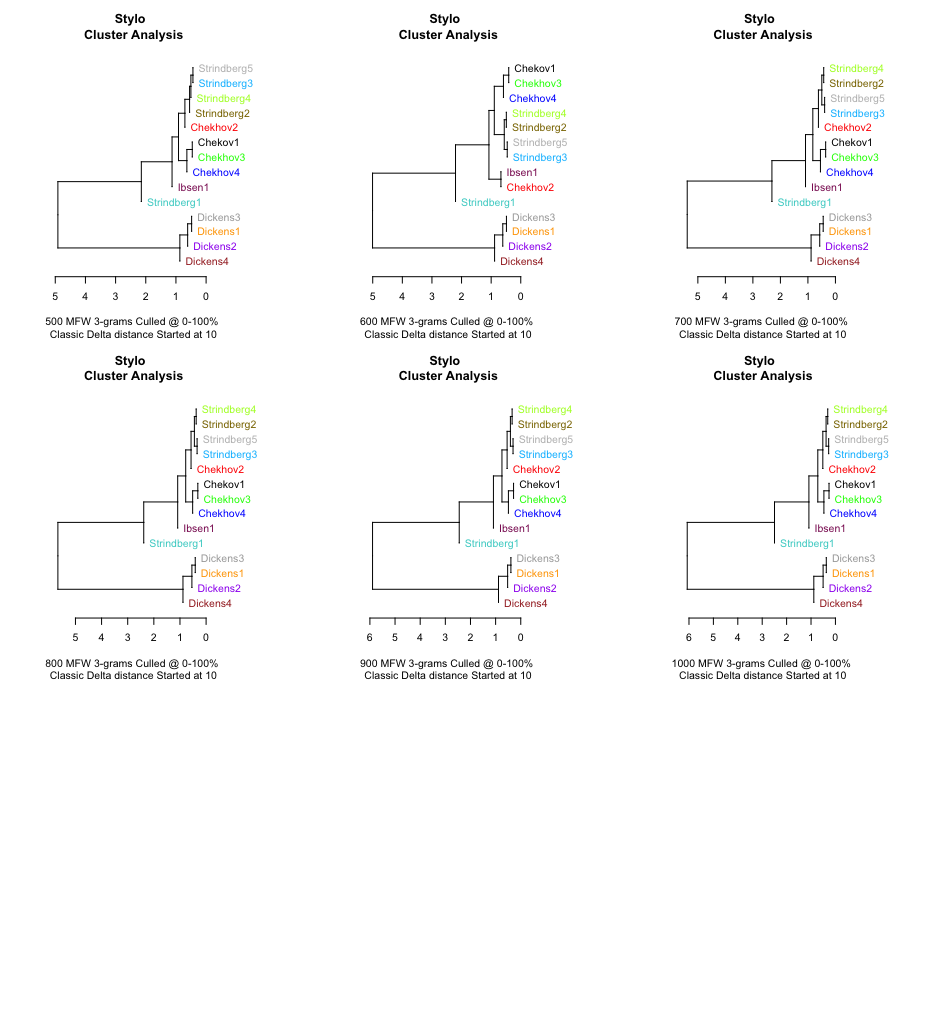
\includegraphics[width=0.9\textwidth]{ChangingMFW.png}
\end{frame}

\begin{frame}
\frametitle{Bootstrap Consensus Trees (BCT)}
%one slide on bootstrap consensus trees
\begin{itemize}
\item Idea: 
\begin{enumerate}
\item Build multiple hierarchical clusters of the corpus following a bootstrapping procedure, using a sample of data each time. 
\item Eventually, keep only those groupings that are seen at least X\% of times in the process. 
\end{enumerate}
\item So, if I choose X as 50\%, it means that in my final grouping, I choose only those groups whose elements are seen at least 50\% of the times in the dendrograms I constructed. 
\item This is an alternative to building a single hierarchical cluster, as this decides its grouping after looking multiple clusters.
\end{itemize}
\end{frame}


\begin{frame}
\frametitle{BCT in action}
\small
\url{https://sites.google.com/site/computationalstylistics/projects/lee_vs_capote}
\end{frame}



\begin{frame}
\frametitle{Rolling Delta}
\begin{itemize}
\item Burrow's delta method, extended to visualize stylistic shifts within a single text. \pause
\item Idea:
\begin{itemize}	
\item Break up each text into equally sized, partially overlapping samples using two parameters - window size, step size.
\item If  we  specify  a window  size? of  5,000  and  a  step  size  of  100, the  first  sample  of  a  text  contains1-5000 words of the text, second sample contains: 101-5101 words, and so on. 
\item Let us say I want to take only the n most frequent words as my "features" for doing this.
\end{itemize}
\end{itemize}
\end{frame}

\begin{frame}
\frametitle{Rolling Delta - continued}
\begin{itemize}
\item For each "reference text", we compute a "centroid" vector of size n where each element represents the mean frequency for a word in all those samples of a text.
\item We also keep track of the standard deviations for these n words in this reference text.
\item When we get a new test document, we split that into samples as before, and use the following formula to get the "delta" of each sample:
\\ $\Delta(C,W) = \Sigma_{i=1}^n \frac{1}{\sigma_i (C)} |\mu_i(C)-f_i(W)|$
\item This is then plotted along with the reference text.
\end{itemize}
\end{frame}

\begin{frame}
\frametitle{Rolling Delta - student projects}
\small
\url{https://sites.google.com/site/computationalstylistics/projects/testing-rolling-delta}
\end{frame}


%Other functions in stylo.
\begin{frame}
\frametitle{Other Functions in Stylo}
\begin{itemize}
\item text classification
\item principal component analysis
\item ... 
\end{itemize}
\end{frame}

\begin{frame}
\frametitle{}
\Large Beyond stylometry - one application with stylo
\end{frame}

\begin{frame}
\frametitle{in what other scenario can Stylo visualizations be useful?}
\framesubtitle{my project from 2016}
\begin{itemize}
\item Data we had: 
\begin{itemize}
\item TOEFL essays written by people with different native language backgrounds (L1) in English (L2).
\item Size: 8830 essays in total, 11 L1s, 2 proficiency levels (medium, high)
\item 11 L1s: CHI, JPN, KOR, TEL, HIN, ARA, TUR, GER, ITA, SPA, FRE.
\end{itemize}
\item Question we explored: ow far is visualization useful in forming hypotheses about the relationship between L1 and L2 proficiency?
\end{itemize}
\end{frame}

\begin{frame}
\frametitle{Methods: used Stylo}
\begin{itemize}
\item Word, Character and POS n-grams (uni, bi, tri grams)
\item Experimented with different frequencies (100 Most frequent n-grams to 1000 most frequent n-grams)
\item Experimented with culling (how many n-grams in the final ones considered appear in how many text categories)
\end{itemize}
Pre-processing: only lowercasing and tokenizing. POS tagging was done with Stanford Tagger. 
\end{frame}

\begin{frame}
\frametitle{Bootstrap Consensus Tree}
  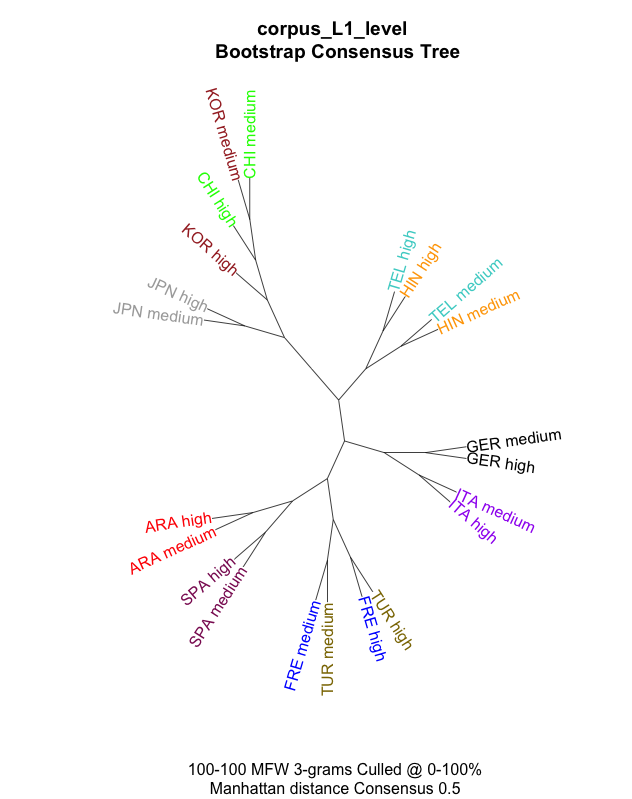
\includegraphics[width=.7\textwidth]{alt1.png}
\end{frame}

\begin{frame}
\frametitle{PCA-1}
  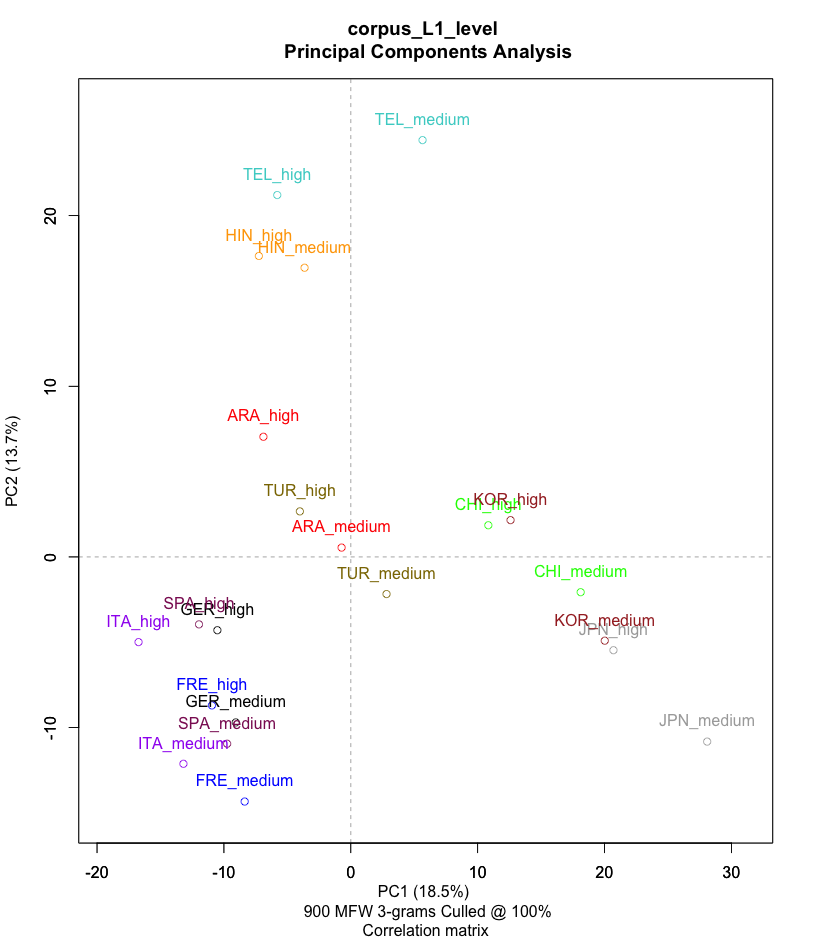
\includegraphics[width=.7\textwidth]{alt2.png}
\end{frame}

\begin{frame}
\frametitle{PCA-2}
  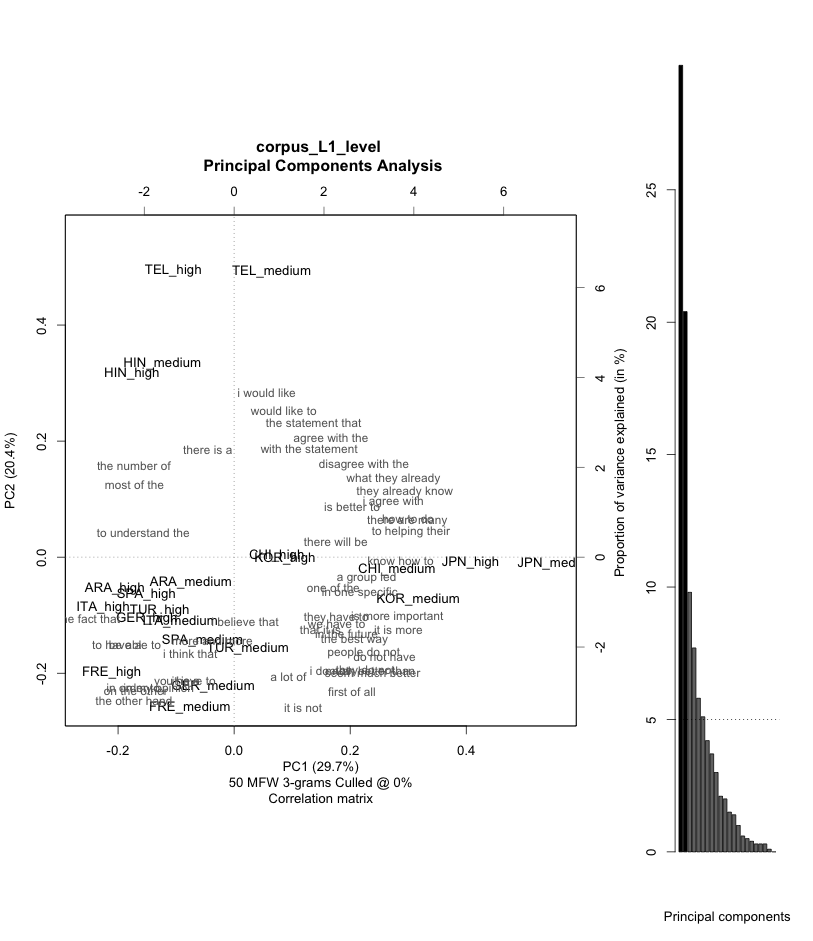
\includegraphics[width=.7\textwidth]{alt3.png}
\end{frame}

\begin{frame}
\frametitle{Next Class}
\begin{itemize}
\item exercises with stylo/wordcloud/topicmodels
\item or working on your final projects etc.
\item Attendance question for today: Think of some scenarios where stylo can be a useful library for the kind of data you want to analyze in your disciplines?
\end{itemize}
\end{frame}

\end{document}

